\chapter{Non-standard evaluation}\label{nse}

\begin{quote}
``Flexibility in syntax, if it does not lead to ambiguity, would seem a
reasonable thing to ask of an interactive programming language.''

--- Kent Pitman
\end{quote}

R has powerful tools for computing not only on values, but also on the
actions that lead to those values. If you're coming from another
programming language, they are one of the most surprising features of R.
Consider the following simple snippet of code that plots a sine curve:

\begin{Shaded}
\begin{Highlighting}[]
\NormalTok{x <-}\StringTok{ }\KeywordTok{seq}\NormalTok{(}\DecValTok{0}\NormalTok{, }\DecValTok{2} \NormalTok{*}\StringTok{ }\NormalTok{pi, }\DataTypeTok{length =} \DecValTok{100}\NormalTok{)}
\NormalTok{sinx <-}\StringTok{ }\KeywordTok{sin}\NormalTok{(x)}
\KeywordTok{plot}\NormalTok{(x, sinx, }\DataTypeTok{type =} \StringTok{"l"}\NormalTok{)}
\end{Highlighting}
\end{Shaded}

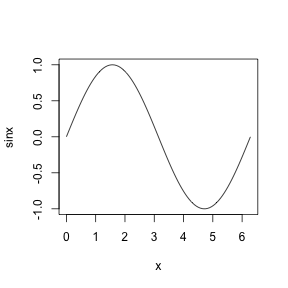
\includegraphics{figures/plot-labels.pdf}

Look at the labels on the axes. How did R know that the variable on the
x axis is called \texttt{x} and the variable on the y axis is called
\texttt{sinx}? In most programming languages, you can only access the
values of a function's arguments. In R, you can also access the code
used to compute them. This makes it possible to evaluate code in
non-standard ways: to use what is known as \textbf{non-standard
evaluation}, or NSE for short. NSE is particularly useful for functions
when doing interactive data analysis because it can dramatically reduce
the amount of typing. \index{non-standard evaluation}

\paragraph{Outline}

\begin{itemize}
\item
  \hyperref[capturing-expressions]{Capturing expressions} teaches you
  how to capture unevaluated expressions using \texttt{substitute()}.
\item
  \hyperref[subset]{Non-standard evaluation} shows you \texttt{subset()}
  works with combining \texttt{substitute()} with \texttt{eval()} to
  allow you to succinctly select rows from a data frame.
\item
  \hyperref[scoping-issues]{Scoping issues} discusses scoping issues
  specific to NSE, and will show you how to resolve them.
\item
  \hyperref[calling-from-another-function]{Calling from another
  function} shows why every function that uses NSE should have an escape
  hatch, a version that uses regular evaluation.
\item
  \hyperref[substitute]{Substitute} teaches you how to use
  \texttt{substitute()} to work with functions that don't have an escape
  hatch.
\item
  \hyperref[nse-downsides]{The downsides} finishes off the chapter with
  a discussion of the downsides of NSE.
\end{itemize}

\paragraph{Prerequisites}

Before reading this chapter, make sure you're familiar with environments
(\hyperref[environments]{Environments}) and lexical scoping
(\hyperref[lexical-scoping]{Lexical scoping}). You'll also need to
install the pryr package with \texttt{install.packages("pryr")}. Some
exercises require the plyr package, which you can install from CRAN with
\texttt{install.packages("plyr")}.

\hyperdef{}{capturing-expressions}{\section{Capturing
expressions}\label{capturing-expressions}}

\texttt{substitute()} makes non-standard evaluation possible. It looks
at a function argument and instead of seeing the value, it sees the code
used to compute the value: \indexc{substitute()}

\begin{Shaded}
\begin{Highlighting}[]
\NormalTok{f <-}\StringTok{ }\NormalTok{function(x) \{}
  \KeywordTok{substitute}\NormalTok{(x)}
\NormalTok{\}}
\KeywordTok{f}\NormalTok{(}\DecValTok{1}\NormalTok{:}\DecValTok{10}\NormalTok{)}
\CommentTok{#> 1:10}

\NormalTok{x <-}\StringTok{ }\DecValTok{10}
\KeywordTok{f}\NormalTok{(x)}
\CommentTok{#> x}

\NormalTok{y <-}\StringTok{ }\DecValTok{13}
\KeywordTok{f}\NormalTok{(x +}\StringTok{ }\NormalTok{y^}\DecValTok{2}\NormalTok{)}
\CommentTok{#> x + y^2}
\end{Highlighting}
\end{Shaded}

For now, we won't worry about exactly what \texttt{substitute()} returns
(that's the topic of \hyperref[metaprogramming]{the following chapter}),
but we'll call it an expression.

\texttt{substitute()} works because function arguments are represented
by a special type of object called a \textbf{promise}. A promise
captures the expression needed to compute the value and the environment
in which to compute it. You're not normally aware of promises because
the first time you access a promise its code is evaluated in its
environment, yielding a value. \index{promises}

\texttt{substitute()} is often paired with \texttt{deparse()}. That
function takes the result of \texttt{substitute()}, an expression, and
turns it into a character vector. \indexc{deparse()}

\begin{Shaded}
\begin{Highlighting}[]
\NormalTok{g <-}\StringTok{ }\NormalTok{function(x) }\KeywordTok{deparse}\NormalTok{(}\KeywordTok{substitute}\NormalTok{(x))}
\KeywordTok{g}\NormalTok{(}\DecValTok{1}\NormalTok{:}\DecValTok{10}\NormalTok{)}
\CommentTok{#> [1] "1:10"}
\KeywordTok{g}\NormalTok{(x)}
\CommentTok{#> [1] "x"}
\KeywordTok{g}\NormalTok{(x +}\StringTok{ }\NormalTok{y^}\DecValTok{2}\NormalTok{)}
\CommentTok{#> [1] "x + y^2"}
\end{Highlighting}
\end{Shaded}

There are a lot of functions in Base R that use these ideas. Some use
them to avoid quotes:

\begin{Shaded}
\begin{Highlighting}[]
\KeywordTok{library}\NormalTok{(ggplot2)}
\CommentTok{# the same as}
\KeywordTok{library}\NormalTok{(}\StringTok{"ggplot2"}\NormalTok{)}
\end{Highlighting}
\end{Shaded}

Other functions, like \texttt{plot.default()}, use them to provide
default labels. \texttt{data.frame()} labels variables with the
expression used to compute them:

\begin{Shaded}
\begin{Highlighting}[]
\NormalTok{x <-}\StringTok{ }\DecValTok{1}\NormalTok{:}\DecValTok{4}
\NormalTok{y <-}\StringTok{ }\NormalTok{letters[}\DecValTok{1}\NormalTok{:}\DecValTok{4}\NormalTok{]}
\KeywordTok{names}\NormalTok{(}\KeywordTok{data.frame}\NormalTok{(x, y))}
\CommentTok{#> [1] "x" "y"}
\end{Highlighting}
\end{Shaded}

We'll learn about the ideas that underlie all these examples by looking
at one particularly useful application of NSE: \texttt{subset()}.

\subsection{Exercises}

\begin{enumerate}
\def\labelenumi{\arabic{enumi}.}
\item
  One important feature of \texttt{deparse()} to be aware of when
  programming is that it can return multiple strings if the input is too
  long. For example, the following call produces a vector of length two:

\begin{Shaded}
\begin{Highlighting}[]
\KeywordTok{g}\NormalTok{(a +}\StringTok{ }\NormalTok{b +}\StringTok{ }\NormalTok{c +}\StringTok{ }\NormalTok{d +}\StringTok{ }\NormalTok{e +}\StringTok{ }\NormalTok{f +}\StringTok{ }\NormalTok{g +}\StringTok{ }\NormalTok{h +}\StringTok{ }\NormalTok{i +}\StringTok{ }\NormalTok{j +}\StringTok{ }\NormalTok{k +}\StringTok{ }\NormalTok{l +}\StringTok{ }\NormalTok{m +}
\StringTok{  }\NormalTok{n +}\StringTok{ }\NormalTok{o +}\StringTok{ }\NormalTok{p +}\StringTok{ }\NormalTok{q +}\StringTok{ }\NormalTok{r +}\StringTok{ }\NormalTok{s +}\StringTok{ }\NormalTok{t +}\StringTok{ }\NormalTok{u +}\StringTok{ }\NormalTok{v +}\StringTok{ }\NormalTok{w +}\StringTok{ }\NormalTok{x +}\StringTok{ }\NormalTok{y +}\StringTok{ }\NormalTok{z)}
\end{Highlighting}
\end{Shaded}

  Why does this happen? Carefully read the documentation. Can you write
  a wrapper around \texttt{deparse()} so that it always returns a single
  string?
\item
  Why does \texttt{as.Date.default()} use \texttt{substitute()} and
  \texttt{deparse()}? Why does \texttt{pairwise.t.test()} use them? Read
  the source code.
\item
  \texttt{pairwise.t.test()} assumes that \texttt{deparse()} always
  returns a length one character vector. Can you construct an input that
  violates this expectation? What happens?
\item
  \texttt{f()}, defined above, just calls \texttt{substitute()}. Why
  can't we use it to define \texttt{g()}? In other words, what will the
  following code return? First make a prediction. Then run the code and
  think about the results.

\begin{Shaded}
\begin{Highlighting}[]
\NormalTok{f <-}\StringTok{ }\NormalTok{function(x) }\KeywordTok{substitute}\NormalTok{(x)}
\NormalTok{g <-}\StringTok{ }\NormalTok{function(x) }\KeywordTok{deparse}\NormalTok{(}\KeywordTok{f}\NormalTok{(x))}
\KeywordTok{g}\NormalTok{(}\DecValTok{1}\NormalTok{:}\DecValTok{10}\NormalTok{)}
\KeywordTok{g}\NormalTok{(x)}
\KeywordTok{g}\NormalTok{(x +}\StringTok{ }\NormalTok{y ^}\StringTok{ }\DecValTok{2} \NormalTok{/}\StringTok{ }\NormalTok{z +}\StringTok{ }\KeywordTok{exp}\NormalTok{(a *}\StringTok{ }\KeywordTok{sin}\NormalTok{(b)))}
\end{Highlighting}
\end{Shaded}
\end{enumerate}

\hyperdef{}{subset}{\section{Non-standard evaluation in
subset}\label{subset}}

While printing out the code supplied to an argument value can be useful,
we can actually do more with the unevaluated code. Take
\texttt{subset()}, for example. It's a useful interactive shortcut for
subsetting data frames: instead of repeating the name of data frame many
times, you can save some typing: \indexc{subset()}

\begin{Shaded}
\begin{Highlighting}[]
\NormalTok{sample_df <-}\StringTok{ }\KeywordTok{data.frame}\NormalTok{(}\DataTypeTok{a =} \DecValTok{1}\NormalTok{:}\DecValTok{5}\NormalTok{, }\DataTypeTok{b =} \DecValTok{5}\NormalTok{:}\DecValTok{1}\NormalTok{, }\DataTypeTok{c =} \KeywordTok{c}\NormalTok{(}\DecValTok{5}\NormalTok{, }\DecValTok{3}\NormalTok{, }\DecValTok{1}\NormalTok{, }\DecValTok{4}\NormalTok{, }\DecValTok{1}\NormalTok{))}

\KeywordTok{subset}\NormalTok{(sample_df, a >=}\StringTok{ }\DecValTok{4}\NormalTok{)}
\CommentTok{#>   a b c}
\CommentTok{#> 4 4 2 4}
\CommentTok{#> 5 5 1 1}
\CommentTok{# equivalent to:}
\CommentTok{# sample_df[sample_df$a >= 4, ]}

\KeywordTok{subset}\NormalTok{(sample_df, b ==}\StringTok{ }\NormalTok{c)}
\CommentTok{#>   a b c}
\CommentTok{#> 1 1 5 5}
\CommentTok{#> 5 5 1 1}
\CommentTok{# equivalent to:}
\CommentTok{# sample_df[sample_df$b == sample_df$c, ]}
\end{Highlighting}
\end{Shaded}

\texttt{subset()} is special because it implements different scoping
rules: the expressions \texttt{a \textgreater{}= 4} or \texttt{b == c}
are evaluated in the specified data frame rather than in the current or
global environments. This is the essence of non-standard evaluation.

How does \texttt{subset()} work? We've already seen how to capture an
argument's expression rather than its result, so we just need to figure
out how to evaluate that expression in the right context. Specifically,
we want \texttt{x} to be interpreted as \texttt{sample\_df\$x}, not
\texttt{globalenv()\$x}. To do this, we need \texttt{eval()}. This
function takes an expression and evaluates it in the specified
environment. \indexc{eval()}

Before we can explore \texttt{eval()}, we need one more useful function:
\texttt{quote()}. It captures an unevaluated expression like
\texttt{substitute()}, but doesn't do any of the advanced
transformations that can make \texttt{substitute()} confusing.
\texttt{quote()} always returns its input as is: \indexc{quote()}
\index{quoting}

\begin{Shaded}
\begin{Highlighting}[]
\KeywordTok{quote}\NormalTok{(}\DecValTok{1}\NormalTok{:}\DecValTok{10}\NormalTok{)}
\CommentTok{#> 1:10}
\KeywordTok{quote}\NormalTok{(x)}
\CommentTok{#> x}
\KeywordTok{quote}\NormalTok{(x +}\StringTok{ }\NormalTok{y^}\DecValTok{2}\NormalTok{)}
\CommentTok{#> x + y^2}
\end{Highlighting}
\end{Shaded}

We need \texttt{quote()} to experiment with \texttt{eval()} because
\texttt{eval()}'s first argument is an expression. So if you only
provide one argument, it will evaluate the expression in the current
environment. This makes \texttt{eval(quote(x))} exactly equivalent to
\texttt{x}, regardless of what \texttt{x} is:

\begin{Shaded}
\begin{Highlighting}[]
\KeywordTok{eval}\NormalTok{(}\KeywordTok{quote}\NormalTok{(x <-}\StringTok{ }\DecValTok{1}\NormalTok{))}
\KeywordTok{eval}\NormalTok{(}\KeywordTok{quote}\NormalTok{(x))}
\CommentTok{#> [1] 1}

\KeywordTok{eval}\NormalTok{(}\KeywordTok{quote}\NormalTok{(y))}
\CommentTok{#> Error: object 'y' not found}
\end{Highlighting}
\end{Shaded}

\texttt{quote()} and \texttt{eval()} are opposites. In the example
below, each \texttt{eval()} peels off one layer of \texttt{quote()}'s.

\begin{Shaded}
\begin{Highlighting}[]
\KeywordTok{quote}\NormalTok{(}\DecValTok{2} \NormalTok{+}\StringTok{ }\DecValTok{2}\NormalTok{)}
\CommentTok{#> 2 + 2}
\KeywordTok{eval}\NormalTok{(}\KeywordTok{quote}\NormalTok{(}\DecValTok{2} \NormalTok{+}\StringTok{ }\DecValTok{2}\NormalTok{))}
\CommentTok{#> [1] 4}

\KeywordTok{quote}\NormalTok{(}\KeywordTok{quote}\NormalTok{(}\DecValTok{2} \NormalTok{+}\StringTok{ }\DecValTok{2}\NormalTok{))}
\CommentTok{#> quote(2 + 2)}
\KeywordTok{eval}\NormalTok{(}\KeywordTok{quote}\NormalTok{(}\KeywordTok{quote}\NormalTok{(}\DecValTok{2} \NormalTok{+}\StringTok{ }\DecValTok{2}\NormalTok{)))}
\CommentTok{#> 2 + 2}
\KeywordTok{eval}\NormalTok{(}\KeywordTok{eval}\NormalTok{(}\KeywordTok{quote}\NormalTok{(}\KeywordTok{quote}\NormalTok{(}\DecValTok{2} \NormalTok{+}\StringTok{ }\DecValTok{2}\NormalTok{))))}
\CommentTok{#> [1] 4}
\end{Highlighting}
\end{Shaded}

\texttt{eval()}'s second argument specifies the environment in which the
code is executed:

\begin{Shaded}
\begin{Highlighting}[]
\NormalTok{x <-}\StringTok{ }\DecValTok{10}
\KeywordTok{eval}\NormalTok{(}\KeywordTok{quote}\NormalTok{(x))}
\CommentTok{#> [1] 10}

\NormalTok{e <-}\StringTok{ }\KeywordTok{new.env}\NormalTok{()}
\NormalTok{e$x <-}\StringTok{ }\DecValTok{20}
\KeywordTok{eval}\NormalTok{(}\KeywordTok{quote}\NormalTok{(x), e)}
\CommentTok{#> [1] 20}
\end{Highlighting}
\end{Shaded}

Because lists and data frames bind names to values in a similar way to
environments, \texttt{eval()}'s second argument need not be limited to
an environment: it can also be a list or a data frame.

\begin{Shaded}
\begin{Highlighting}[]
\KeywordTok{eval}\NormalTok{(}\KeywordTok{quote}\NormalTok{(x), }\KeywordTok{list}\NormalTok{(}\DataTypeTok{x =} \DecValTok{30}\NormalTok{))}
\CommentTok{#> [1] 30}
\KeywordTok{eval}\NormalTok{(}\KeywordTok{quote}\NormalTok{(x), }\KeywordTok{data.frame}\NormalTok{(}\DataTypeTok{x =} \DecValTok{40}\NormalTok{))}
\CommentTok{#> [1] 40}
\end{Highlighting}
\end{Shaded}

This gives us one part of \texttt{subset()}:

\begin{Shaded}
\begin{Highlighting}[]
\KeywordTok{eval}\NormalTok{(}\KeywordTok{quote}\NormalTok{(a >=}\StringTok{ }\DecValTok{4}\NormalTok{), sample_df)}
\CommentTok{#> [1] FALSE FALSE FALSE  TRUE  TRUE}
\KeywordTok{eval}\NormalTok{(}\KeywordTok{quote}\NormalTok{(b ==}\StringTok{ }\NormalTok{c), sample_df)}
\CommentTok{#> [1]  TRUE FALSE FALSE FALSE  TRUE}
\end{Highlighting}
\end{Shaded}

A common mistake when using \texttt{eval()} is to forget to quote the
first argument. Compare the results below:

\begin{Shaded}
\begin{Highlighting}[]
\NormalTok{a <-}\StringTok{ }\DecValTok{10}
\KeywordTok{eval}\NormalTok{(}\KeywordTok{quote}\NormalTok{(a), sample_df)}
\CommentTok{#> [1] 1 2 3 4 5}
\KeywordTok{eval}\NormalTok{(a, sample_df)}
\CommentTok{#> [1] 10}

\KeywordTok{eval}\NormalTok{(}\KeywordTok{quote}\NormalTok{(b), sample_df)}
\CommentTok{#> [1] 5 4 3 2 1}
\KeywordTok{eval}\NormalTok{(b, sample_df)}
\CommentTok{#> Error: object 'b' not found}
\end{Highlighting}
\end{Shaded}

We can use \texttt{eval()} and \texttt{substitute()} to write
\texttt{subset()}. We first capture the call representing the condition,
then we evaluate it in the context of the data frame and, finally, we
use the result for subsetting:

\begin{Shaded}
\begin{Highlighting}[]
\NormalTok{subset2 <-}\StringTok{ }\NormalTok{function(x, condition) \{}
  \NormalTok{condition_call <-}\StringTok{ }\KeywordTok{substitute}\NormalTok{(condition)}
  \NormalTok{r <-}\StringTok{ }\KeywordTok{eval}\NormalTok{(condition_call, x)}
  \NormalTok{x[r, ]}
\NormalTok{\}}
\KeywordTok{subset2}\NormalTok{(sample_df, a >=}\StringTok{ }\DecValTok{4}\NormalTok{)}
\CommentTok{#>   a b c}
\CommentTok{#> 4 4 2 4}
\CommentTok{#> 5 5 1 1}
\end{Highlighting}
\end{Shaded}

\subsection{Exercises}

\begin{enumerate}
\def\labelenumi{\arabic{enumi}.}
\item
  Predict the results of the following lines of code:

\begin{Shaded}
\begin{Highlighting}[]
\KeywordTok{eval}\NormalTok{(}\KeywordTok{quote}\NormalTok{(}\KeywordTok{eval}\NormalTok{(}\KeywordTok{quote}\NormalTok{(}\KeywordTok{eval}\NormalTok{(}\KeywordTok{quote}\NormalTok{(}\DecValTok{2} \NormalTok{+}\StringTok{ }\DecValTok{2}\NormalTok{))))))}
\KeywordTok{eval}\NormalTok{(}\KeywordTok{eval}\NormalTok{(}\KeywordTok{quote}\NormalTok{(}\KeywordTok{eval}\NormalTok{(}\KeywordTok{quote}\NormalTok{(}\KeywordTok{eval}\NormalTok{(}\KeywordTok{quote}\NormalTok{(}\DecValTok{2} \NormalTok{+}\StringTok{ }\DecValTok{2}\NormalTok{)))))))}
\KeywordTok{quote}\NormalTok{(}\KeywordTok{eval}\NormalTok{(}\KeywordTok{quote}\NormalTok{(}\KeywordTok{eval}\NormalTok{(}\KeywordTok{quote}\NormalTok{(}\KeywordTok{eval}\NormalTok{(}\KeywordTok{quote}\NormalTok{(}\DecValTok{2} \NormalTok{+}\StringTok{ }\DecValTok{2}\NormalTok{)))))))}
\end{Highlighting}
\end{Shaded}
\item
  \texttt{subset2()} has a bug if you use it with a single column data
  frame. What should the following code return? How can you modify
  \texttt{subset2()} so it returns the correct type of object?

\begin{Shaded}
\begin{Highlighting}[]
\NormalTok{sample_df2 <-}\StringTok{ }\KeywordTok{data.frame}\NormalTok{(}\DataTypeTok{x =} \DecValTok{1}\NormalTok{:}\DecValTok{10}\NormalTok{)}
\KeywordTok{subset2}\NormalTok{(sample_df2, x >}\StringTok{ }\DecValTok{8}\NormalTok{)}
\CommentTok{#> [1]  9 10}
\end{Highlighting}
\end{Shaded}
\item
  The real subset function (\texttt{subset.data.frame()}) removes
  missing values in the condition. Modify \texttt{subset2()} to do the
  same: drop the offending rows.
\item
  What happens if you use \texttt{quote()} instead of
  \texttt{substitute()} inside of \texttt{subset2()}?
\item
  The second argument in \texttt{subset()} allows you to select
  variables. It treats variable names as if they were positions. This
  allows you to do things like \texttt{subset(mtcars, , -cyl)} to drop
  the cylinder variable, or \texttt{subset(mtcars, , disp:drat)} to
  select all the variables between \texttt{disp} and \texttt{drat}. How
  does this work? I've made this easier to understand by extracting it
  out into its own function.

\begin{Shaded}
\begin{Highlighting}[]
\NormalTok{select <-}\StringTok{ }\NormalTok{function(df, vars) \{}
  \NormalTok{vars <-}\StringTok{ }\KeywordTok{substitute}\NormalTok{(vars)}
  \NormalTok{var_pos <-}\StringTok{ }\KeywordTok{setNames}\NormalTok{(}\KeywordTok{as.list}\NormalTok{(}\KeywordTok{seq_along}\NormalTok{(df)), }\KeywordTok{names}\NormalTok{(df))}
  \NormalTok{pos <-}\StringTok{ }\KeywordTok{eval}\NormalTok{(vars, var_pos)}
  \NormalTok{df[, pos, drop =}\StringTok{ }\OtherTok{FALSE}\NormalTok{]}
\NormalTok{\}}
\KeywordTok{select}\NormalTok{(mtcars, -cyl)}
\end{Highlighting}
\end{Shaded}
\item
  What does \texttt{evalq()} do? Use it to reduce the amount of typing
  for the examples above that use both \texttt{eval()} and
  \texttt{quote()}.
\end{enumerate}

\hyperdef{}{scoping-issues}{\section{Scoping
issues}\label{scoping-issues}}

It certainly looks like our \texttt{subset2()} function works. But since
we're working with expressions instead of values, we need to test things
more extensively. For example, the following applications of
\texttt{subset2()} should all return the same value because the only
difference between them is the name of a variable:
\index{lexical scoping}

\begin{Shaded}
\begin{Highlighting}[]
\NormalTok{y <-}\StringTok{ }\DecValTok{4}
\NormalTok{x <-}\StringTok{ }\DecValTok{4}
\NormalTok{condition <-}\StringTok{ }\DecValTok{4}
\NormalTok{condition_call <-}\StringTok{ }\DecValTok{4}

\KeywordTok{subset2}\NormalTok{(sample_df, a ==}\StringTok{ }\DecValTok{4}\NormalTok{)}
\CommentTok{#>   a b c}
\CommentTok{#> 4 4 2 4}
\KeywordTok{subset2}\NormalTok{(sample_df, a ==}\StringTok{ }\NormalTok{y)}
\CommentTok{#>   a b c}
\CommentTok{#> 4 4 2 4}
\KeywordTok{subset2}\NormalTok{(sample_df, a ==}\StringTok{ }\NormalTok{x)}
\CommentTok{#>       a  b  c}
\CommentTok{#> 1     1  5  5}
\CommentTok{#> 2     2  4  3}
\CommentTok{#> 3     3  3  1}
\CommentTok{#> 4     4  2  4}
\CommentTok{#> 5     5  1  1}
\CommentTok{#> NA   NA NA NA}
\CommentTok{#> NA.1 NA NA NA}
\KeywordTok{subset2}\NormalTok{(sample_df, a ==}\StringTok{ }\NormalTok{condition)}
\CommentTok{#> Error: object 'a' not found}
\KeywordTok{subset2}\NormalTok{(sample_df, a ==}\StringTok{ }\NormalTok{condition_call)}
\CommentTok{#> Warning: longer object length is not a multiple of shorter}
\CommentTok{#> object length}
\CommentTok{#> [1] a b c}
\CommentTok{#> <0 rows> (or 0-length row.names)}
\end{Highlighting}
\end{Shaded}

What went wrong? You can get a hint from the variable names I've chosen:
they are all names of variables defined inside \texttt{subset2()}. If
\texttt{eval()} can't find the variable inside the data frame (its
second argument), it looks in the environment of \texttt{subset2()}.
That's obviously not what we want, so we need some way to tell
\texttt{eval()} where to look if it can't find the variables in the data
frame.

The key is the third argument to \texttt{eval()}: \texttt{enclos}. This
allows us to specify a parent (or enclosing) environment for objects
that don't have one (like lists and data frames). If the binding is not
found in \texttt{env}, \texttt{eval()} will next look in
\texttt{enclos}, and then in the parents of \texttt{enclos}.
\texttt{enclos} is ignored if \texttt{env} is a real environment. We
want to look for \texttt{x} in the environment from which
\texttt{subset2()} was called. In R terminology this is called the
\textbf{parent frame} and is accessed with \texttt{parent.frame()}. This
is an example of
\href{http://en.wikipedia.org/wiki/Scope_\%28programming\%29\#Dynamic_scoping}{dynamic
scope}: the values come from the location where the function was called,
not where it was defined. \indexc{parent.frame()}

With this modification our function now works:

\begin{Shaded}
\begin{Highlighting}[]
\NormalTok{subset2 <-}\StringTok{ }\NormalTok{function(x, condition) \{}
  \NormalTok{condition_call <-}\StringTok{ }\KeywordTok{substitute}\NormalTok{(condition)}
  \NormalTok{r <-}\StringTok{ }\KeywordTok{eval}\NormalTok{(condition_call, x, }\KeywordTok{parent.frame}\NormalTok{())}
  \NormalTok{x[r, ]}
\NormalTok{\}}

\NormalTok{x <-}\StringTok{ }\DecValTok{4}
\KeywordTok{subset2}\NormalTok{(sample_df, a ==}\StringTok{ }\NormalTok{x)}
\CommentTok{#>   a b c}
\CommentTok{#> 4 4 2 4}
\end{Highlighting}
\end{Shaded}

Using \texttt{enclos} is just a shortcut for converting a list or data
frame to an environment. We can get the same behaviour by using
\texttt{list2env()}. It turns a list into an environment with an
explicit parent: \indexc{list2env()}

\begin{Shaded}
\begin{Highlighting}[]
\NormalTok{subset2a <-}\StringTok{ }\NormalTok{function(x, condition) \{}
  \NormalTok{condition_call <-}\StringTok{ }\KeywordTok{substitute}\NormalTok{(condition)}
  \NormalTok{env <-}\StringTok{ }\KeywordTok{list2env}\NormalTok{(x, }\DataTypeTok{parent =} \KeywordTok{parent.frame}\NormalTok{())}
  \NormalTok{r <-}\StringTok{ }\KeywordTok{eval}\NormalTok{(condition_call, env)}
  \NormalTok{x[r, ]}
\NormalTok{\}}

\NormalTok{x <-}\StringTok{ }\DecValTok{5}
\KeywordTok{subset2a}\NormalTok{(sample_df, a ==}\StringTok{ }\NormalTok{x)}
\CommentTok{#>   a b c}
\CommentTok{#> 5 5 1 1}
\end{Highlighting}
\end{Shaded}

\subsection{Exercises}

\begin{enumerate}
\def\labelenumi{\arabic{enumi}.}
\item
  \texttt{plyr::arrange()} works similarly to \texttt{subset()}, but
  instead of selecting rows, it reorders them. How does it work? What
  does \texttt{substitute(order(...))} do? Create a function that does
  only that and experiment with it.
\item
  What does \texttt{transform()} do? Read the documentation. How does it
  work? Read the source code for \texttt{transform.data.frame()}. What
  does \texttt{substitute(list(...))} do?
\item
  \texttt{plyr::mutate()} is similar to \texttt{transform()} but it
  applies the transformations sequentially so that transformation can
  refer to columns that were just created:

\begin{Shaded}
\begin{Highlighting}[]
\NormalTok{df <-}\StringTok{ }\KeywordTok{data.frame}\NormalTok{(}\DataTypeTok{x =} \DecValTok{1}\NormalTok{:}\DecValTok{5}\NormalTok{)}
\KeywordTok{transform}\NormalTok{(df, }\DataTypeTok{x2 =} \NormalTok{x *}\StringTok{ }\NormalTok{x, }\DataTypeTok{x3 =} \NormalTok{x2 *}\StringTok{ }\NormalTok{x)}
\NormalTok{plyr::}\KeywordTok{mutate}\NormalTok{(df, }\DataTypeTok{x2 =} \NormalTok{x *}\StringTok{ }\NormalTok{x, }\DataTypeTok{x3 =} \NormalTok{x2 *}\StringTok{ }\NormalTok{x)}
\end{Highlighting}
\end{Shaded}

  How does mutate work? What's the key difference between
  \texttt{mutate()} and \texttt{transform()}?
\item
  What does \texttt{with()} do? How does it work? Read the source code
  for \texttt{with.default()}. What does \texttt{within()} do? How does
  it work? Read the source code for \texttt{within.data.frame()}. Why is
  the code so much more complex than \texttt{with()}?
\end{enumerate}

\hyperdef{}{calling-from-another-function}{\section{Calling from another
function}\label{calling-from-another-function}}

Typically, computing on the language is most useful when functions are
called directly by users and less useful when they are called by other
functions. While \texttt{subset()} saves typing, it's actually difficult
to use non-interactively. For example, imagine we want to create a
function that randomly reorders a subset of rows of data. A nice way to
do that would be to compose a function that reorders with another that
selects. Let's try that: \index{non-standard evaluation!escape hatches}

\begin{Shaded}
\begin{Highlighting}[]
\NormalTok{subset2 <-}\StringTok{ }\NormalTok{function(x, condition) \{}
  \NormalTok{condition_call <-}\StringTok{ }\KeywordTok{substitute}\NormalTok{(condition)}
  \NormalTok{r <-}\StringTok{ }\KeywordTok{eval}\NormalTok{(condition_call, x, }\KeywordTok{parent.frame}\NormalTok{())}
  \NormalTok{x[r, ]}
\NormalTok{\}}

\NormalTok{scramble <-}\StringTok{ }\NormalTok{function(x) x[}\KeywordTok{sample}\NormalTok{(}\KeywordTok{nrow}\NormalTok{(x)), ]}

\NormalTok{subscramble <-}\StringTok{ }\NormalTok{function(x, condition) \{}
  \KeywordTok{scramble}\NormalTok{(}\KeywordTok{subset2}\NormalTok{(x, condition))}
\NormalTok{\}}
\end{Highlighting}
\end{Shaded}

But it doesn't work:

\begin{Shaded}
\begin{Highlighting}[]
\KeywordTok{subscramble}\NormalTok{(sample_df, a >=}\StringTok{ }\DecValTok{4}\NormalTok{)}
\CommentTok{# Error in eval(expr, envir, enclos) : object 'a' not found}
\KeywordTok{traceback}\NormalTok{()}
\CommentTok{#> 5: eval(expr, envir, enclos)}
\CommentTok{#> 4: eval(condition_call, x, parent.frame()) at #3}
\CommentTok{#> 3: subset2(x, condition) at #1}
\CommentTok{#> 2: scramble(subset2(x, condition)) at #2}
\CommentTok{#> 1: subscramble(sample_df, a >= 4)}
\end{Highlighting}
\end{Shaded}

What's gone wrong? To figure it out, let us \texttt{debug()} subset2()`
and work through the code line-by-line:

\begin{Shaded}
\begin{Highlighting}[]
\KeywordTok{debugonce}\NormalTok{(subset2)}
\KeywordTok{subscramble}\NormalTok{(sample_df, a >=}\StringTok{ }\DecValTok{4}\NormalTok{)}
\CommentTok{#> debugging in: subset2(x, condition)}
\CommentTok{#> debug at #1: \{}
\CommentTok{#>     condition_call <- substitute(condition)}
\CommentTok{#>     r <- eval(condition_call, x, parent.frame())}
\CommentTok{#>     x[r, ]}
\CommentTok{#> \}}
\NormalTok{n}
\CommentTok{#> debug at #2: condition_call <- substitute(condition)}
\NormalTok{n}
\CommentTok{#> debug at #3: r <- eval(condition_call, x, parent.frame())}
\NormalTok{r <-}\StringTok{ }\KeywordTok{eval}\NormalTok{(condition_call, x, }\KeywordTok{parent.frame}\NormalTok{())}
\CommentTok{#> Error in eval(expr, envir, enclos) : object 'a' not found}
\NormalTok{condition_call}
\CommentTok{#> condition}
\KeywordTok{eval}\NormalTok{(condition_call, x)}
\CommentTok{#> Error in eval(expr, envir, enclos) : object 'a' not found}
\NormalTok{Q}
\end{Highlighting}
\end{Shaded}

Can you see what the problem is? \texttt{condition\_call} contains the
expression \texttt{condition}. So when we evaluate
\texttt{condition\_call} it also evaluates \texttt{condition}, which has
the value \texttt{a \textgreater{}= 4}. However, this can't be computed
because there's no object called \texttt{a} in the parent environment.
But, if \texttt{a} were set in the global environment, even more
confusing things can happen:

\begin{Shaded}
\begin{Highlighting}[]
\NormalTok{a <-}\StringTok{ }\DecValTok{4}
\KeywordTok{subscramble}\NormalTok{(sample_df, a ==}\StringTok{ }\DecValTok{4}\NormalTok{)}
\CommentTok{#>   a b c}
\CommentTok{#> 4 4 2 4}
\CommentTok{#> 3 3 3 1}
\CommentTok{#> 1 1 5 5}
\CommentTok{#> 5 5 1 1}
\CommentTok{#> 2 2 4 3}

\NormalTok{a <-}\StringTok{ }\KeywordTok{c}\NormalTok{(}\DecValTok{1}\NormalTok{, }\DecValTok{1}\NormalTok{, }\DecValTok{4}\NormalTok{, }\DecValTok{4}\NormalTok{, }\DecValTok{4}\NormalTok{, }\DecValTok{4}\NormalTok{)}
\KeywordTok{subscramble}\NormalTok{(sample_df, a >=}\StringTok{ }\DecValTok{4}\NormalTok{)}
\CommentTok{#>     a  b  c}
\CommentTok{#> 5   5  1  1}
\CommentTok{#> NA NA NA NA}
\CommentTok{#> 4   4  2  4}
\CommentTok{#> 3   3  3  1}
\end{Highlighting}
\end{Shaded}

This is an example of the general tension between functions that are
designed for interactive use and functions that are safe to program
with. A function that uses \texttt{substitute()} might reduce typing,
but it can be difficult to call from another function.

As a developer, you should always provide an escape hatch: an
alternative version of the function that uses standard evaluation. In
this case, we could write a version of \texttt{subset2()} that takes an
already quoted expression:

\begin{Shaded}
\begin{Highlighting}[]
\NormalTok{subset2_q <-}\StringTok{ }\NormalTok{function(x, condition) \{}
  \NormalTok{r <-}\StringTok{ }\KeywordTok{eval}\NormalTok{(condition, x, }\KeywordTok{parent.frame}\NormalTok{())}
  \NormalTok{x[r, ]}
\NormalTok{\}}
\end{Highlighting}
\end{Shaded}

Here I use the suffix \texttt{\_q} to indicate that it takes a quoted
expression. Most users won't need this function so the name can be a
little longer.

We can then rewrite both \texttt{subset2()} and \texttt{subscramble()}
to use \texttt{subset2\_q()}:

\begin{Shaded}
\begin{Highlighting}[]
\NormalTok{subset2 <-}\StringTok{ }\NormalTok{function(x, condition) \{}
  \KeywordTok{subset2_q}\NormalTok{(x, }\KeywordTok{substitute}\NormalTok{(condition))}
\NormalTok{\}}

\NormalTok{subscramble <-}\StringTok{ }\NormalTok{function(x, condition) \{}
  \NormalTok{condition <-}\StringTok{ }\KeywordTok{substitute}\NormalTok{(condition)}
  \KeywordTok{scramble}\NormalTok{(}\KeywordTok{subset2_q}\NormalTok{(x, condition))}
\NormalTok{\}}

\KeywordTok{subscramble}\NormalTok{(sample_df, a >=}\StringTok{ }\DecValTok{3}\NormalTok{)}
\CommentTok{#>   a b c}
\CommentTok{#> 5 5 1 1}
\CommentTok{#> 4 4 2 4}
\CommentTok{#> 3 3 3 1}
\KeywordTok{subscramble}\NormalTok{(sample_df, a >=}\StringTok{ }\DecValTok{3}\NormalTok{)}
\CommentTok{#>   a b c}
\CommentTok{#> 3 3 3 1}
\CommentTok{#> 5 5 1 1}
\CommentTok{#> 4 4 2 4}
\end{Highlighting}
\end{Shaded}

Base R functions tend to use a different sort of escape hatch. They
often have an argument that turns off NSE. For example,
\texttt{require()} has \texttt{character.only = TRUE}. I don't think
it's a good idea to use an argument to change the behaviour of another
argument because it makes function calls harder to understand.

\subsection{Exercises}

\begin{enumerate}
\def\labelenumi{\arabic{enumi}.}
\item
  The following R functions all use NSE. For each, describe how it uses
  NSE, and read the documentation to determine its escape hatch.

  \begin{itemize}
  \itemsep1pt\parskip0pt\parsep0pt
  \item
    \texttt{rm()}
  \item
    \texttt{library()} and \texttt{require()}
  \item
    \texttt{substitute()}
  \item
    \texttt{data()}
  \item
    \texttt{data.frame()}
  \end{itemize}
\item
  Base functions \texttt{match.fun()}, \texttt{page()}, and
  \texttt{ls()} all try to automatically determine whether you want
  standard or non-standard evaluation. Each uses a different approach.
  Figure out the essence of each approach then compare and contrast.
\item
  Add an escape hatch to \texttt{plyr::mutate()} by splitting it into
  two functions. One function should capture the unevaluated inputs. The
  other should take a data frame and list of expressions and perform the
  computation.
\item
  What's the escape hatch for \texttt{ggplot2::aes()}? What about
  \texttt{plyr::()}? What do they have in common? What are the
  advantages and disadvantages of their differences?
\item
  The version of \texttt{subset2\_q()} I presented is a simplification
  of real code. Why is the following version better?

\begin{Shaded}
\begin{Highlighting}[]
\NormalTok{subset2_q <-}\StringTok{ }\NormalTok{function(x, cond, }\DataTypeTok{env =} \KeywordTok{parent.frame}\NormalTok{()) \{}
  \NormalTok{r <-}\StringTok{ }\KeywordTok{eval}\NormalTok{(cond, x, env)}
  \NormalTok{x[r, ]}
\NormalTok{\}}
\end{Highlighting}
\end{Shaded}

  Rewrite \texttt{subset2()} and \texttt{subscramble()} to use this
  improved version.
\end{enumerate}

\hyperdef{}{substitute}{\section{Substitute}\label{substitute}}

Most functions that use non-standard evaluation provide an escape hatch.
But what happens if you want to call a function that doesn't have one?
For example, imagine you want to create a lattice graphic given the
names of two variables: \indexc{substitute()}

\begin{Shaded}
\begin{Highlighting}[]
\KeywordTok{library}\NormalTok{(lattice)}
\KeywordTok{xyplot}\NormalTok{(mpg ~}\StringTok{ }\NormalTok{disp, }\DataTypeTok{data =} \NormalTok{mtcars)}

\NormalTok{x <-}\StringTok{ }\KeywordTok{quote}\NormalTok{(mpg)}
\NormalTok{y <-}\StringTok{ }\KeywordTok{quote}\NormalTok{(disp)}
\KeywordTok{xyplot}\NormalTok{(x ~}\StringTok{ }\NormalTok{y, }\DataTypeTok{data =} \NormalTok{mtcars)}
\CommentTok{#> Error: object of type 'symbol' is not subsettable}
\end{Highlighting}
\end{Shaded}

We might turn to \texttt{substitute()} and use it for another purpose:
to modify an expression. Unfortunately \texttt{substitute()} has a
feature that makes modifying calls interactively a bit of a pain. When
run from the global environment, it never does substitutions: in fact,
in this situation it behaves just like \texttt{quote()}:
\index{calls!modifying}

\begin{Shaded}
\begin{Highlighting}[]
\NormalTok{a <-}\StringTok{ }\DecValTok{1}
\NormalTok{b <-}\StringTok{ }\DecValTok{2}
\KeywordTok{substitute}\NormalTok{(a +}\StringTok{ }\NormalTok{b +}\StringTok{ }\NormalTok{z)}
\CommentTok{#> a + b + z}
\end{Highlighting}
\end{Shaded}

However, if you run it inside a function, \texttt{substitute()} does
substitute and leaves everything else as is:

\begin{Shaded}
\begin{Highlighting}[]
\NormalTok{f <-}\StringTok{ }\NormalTok{function() \{}
  \NormalTok{a <-}\StringTok{ }\DecValTok{1}
  \NormalTok{b <-}\StringTok{ }\DecValTok{2}
  \KeywordTok{substitute}\NormalTok{(a +}\StringTok{ }\NormalTok{b +}\StringTok{ }\NormalTok{z)}
\NormalTok{\}}
\KeywordTok{f}\NormalTok{()}
\CommentTok{#> 1 + 2 + z}
\end{Highlighting}
\end{Shaded}

To make it easier to experiment with \texttt{substitute()},
\texttt{pryr} provides the \texttt{subs()} function. It works exactly
the same way as \texttt{substitute()} except it has a shorter name and
it works in the global environment. These two features make
experimentation easier:

\begin{Shaded}
\begin{Highlighting}[]
\NormalTok{a <-}\StringTok{ }\DecValTok{1}
\NormalTok{b <-}\StringTok{ }\DecValTok{2}
\KeywordTok{subs}\NormalTok{(a +}\StringTok{ }\NormalTok{b +}\StringTok{ }\NormalTok{z)}
\CommentTok{#> 1 + 2 + z}
\end{Highlighting}
\end{Shaded}

The second argument (of both \texttt{subs()} and \texttt{substitute()})
can override the use of the current environment, and provide an
alternative via a list of name-value pairs. The following example uses
this technique to show some variations on substituting a string,
variable name, or function call:

\begin{Shaded}
\begin{Highlighting}[]
\KeywordTok{subs}\NormalTok{(a +}\StringTok{ }\NormalTok{b, }\KeywordTok{list}\NormalTok{(}\DataTypeTok{a =} \StringTok{"y"}\NormalTok{))}
\CommentTok{#> "y" + b}
\KeywordTok{subs}\NormalTok{(a +}\StringTok{ }\NormalTok{b, }\KeywordTok{list}\NormalTok{(}\DataTypeTok{a =} \KeywordTok{quote}\NormalTok{(y)))}
\CommentTok{#> y + b}
\KeywordTok{subs}\NormalTok{(a +}\StringTok{ }\NormalTok{b, }\KeywordTok{list}\NormalTok{(}\DataTypeTok{a =} \KeywordTok{quote}\NormalTok{(}\KeywordTok{y}\NormalTok{())))}
\CommentTok{#> y() + b}
\end{Highlighting}
\end{Shaded}

Remember that every action in R is a function call, so we can also
replace \texttt{+} with another function:

\begin{Shaded}
\begin{Highlighting}[]
\KeywordTok{subs}\NormalTok{(a +}\StringTok{ }\NormalTok{b, }\KeywordTok{list}\NormalTok{(}\StringTok{"+"} \NormalTok{=}\StringTok{ }\KeywordTok{quote}\NormalTok{(f)))}
\CommentTok{#> f(a, b)}
\KeywordTok{subs}\NormalTok{(a +}\StringTok{ }\NormalTok{b, }\KeywordTok{list}\NormalTok{(}\StringTok{"+"} \NormalTok{=}\StringTok{ }\KeywordTok{quote}\NormalTok{(}\StringTok{`}\DataTypeTok{*}\StringTok{`}\NormalTok{)))}
\CommentTok{#> a * b}
\end{Highlighting}
\end{Shaded}

You can also make nonsense code:

\begin{Shaded}
\begin{Highlighting}[]
\KeywordTok{subs}\NormalTok{(y <-}\StringTok{ }\NormalTok{y +}\StringTok{ }\DecValTok{1}\NormalTok{, }\KeywordTok{list}\NormalTok{(}\DataTypeTok{y =} \DecValTok{1}\NormalTok{))}
\CommentTok{#> 1 <- 1 + 1}
\end{Highlighting}
\end{Shaded}

Formally, substitution takes place by examining all the names in the
expression. If the name refers to:

\begin{enumerate}
\def\labelenumi{\arabic{enumi}.}
\item
  an ordinary variable, it's replaced by the value of the variable.
\item
  a promise (a function argument), it's replaced by the expression
  associated with the promise.
\item
  \texttt{...}, it's replaced by the contents of \texttt{...}.
\end{enumerate}

Otherwise it's left as is.

We can use this to create the right call to \texttt{xyplot()}:

\begin{Shaded}
\begin{Highlighting}[]
\NormalTok{x <-}\StringTok{ }\KeywordTok{quote}\NormalTok{(mpg)}
\NormalTok{y <-}\StringTok{ }\KeywordTok{quote}\NormalTok{(disp)}
\KeywordTok{subs}\NormalTok{(}\KeywordTok{xyplot}\NormalTok{(x ~}\StringTok{ }\NormalTok{y, }\DataTypeTok{data =} \NormalTok{mtcars))}
\CommentTok{#> xyplot(mpg ~ disp, data = mtcars)}
\end{Highlighting}
\end{Shaded}

It's even simpler inside a function, because we don't need to explicitly
quote the x and y variables (rule 2 above):

\begin{Shaded}
\begin{Highlighting}[]
\NormalTok{xyplot2 <-}\StringTok{ }\NormalTok{function(x, y, }\DataTypeTok{data =} \NormalTok{data) \{}
  \KeywordTok{substitute}\NormalTok{(}\KeywordTok{xyplot}\NormalTok{(x ~}\StringTok{ }\NormalTok{y, }\DataTypeTok{data =} \NormalTok{data))}
\NormalTok{\}}
\KeywordTok{xyplot2}\NormalTok{(mpg, disp, }\DataTypeTok{data =} \NormalTok{mtcars)}
\CommentTok{#> xyplot(mpg ~ disp, data = mtcars)}
\end{Highlighting}
\end{Shaded}

If we include \texttt{...} in the call to substitute, we can add
additional arguments to the call:

\begin{Shaded}
\begin{Highlighting}[]
\NormalTok{xyplot3 <-}\StringTok{ }\NormalTok{function(x, y, ...) \{}
  \KeywordTok{substitute}\NormalTok{(}\KeywordTok{xyplot}\NormalTok{(x ~}\StringTok{ }\NormalTok{y, ...))}
\NormalTok{\}}
\KeywordTok{xyplot3}\NormalTok{(mpg, disp, }\DataTypeTok{data =} \NormalTok{mtcars, }\DataTypeTok{col =} \StringTok{"red"}\NormalTok{, }\DataTypeTok{aspect =} \StringTok{"xy"}\NormalTok{)}
\CommentTok{#> xyplot(mpg ~ disp, data = mtcars, col = "red", aspect = "xy")}
\end{Highlighting}
\end{Shaded}

To create the plot, we'd then \texttt{eval()} this call.

\subsection{Adding an escape hatch to substitute}

\texttt{substitute()} is itself a function that uses non-standard
evaluation and doesn't have an escape hatch. This means we can't use
\texttt{substitute()} if we already have an expression saved in a
variable: \indexc{substitute\_q()}

\begin{Shaded}
\begin{Highlighting}[]
\NormalTok{x <-}\StringTok{ }\KeywordTok{quote}\NormalTok{(a +}\StringTok{ }\NormalTok{b)}
\KeywordTok{substitute}\NormalTok{(x, }\KeywordTok{list}\NormalTok{(}\DataTypeTok{a =} \DecValTok{1}\NormalTok{, }\DataTypeTok{b =} \DecValTok{2}\NormalTok{))}
\CommentTok{#> x}
\end{Highlighting}
\end{Shaded}

Although \texttt{substitute()} doesn't have a built-in escape hatch, we
can use the function itself to create one:

\begin{Shaded}
\begin{Highlighting}[]
\NormalTok{substitute_q <-}\StringTok{ }\NormalTok{function(x, env) \{}
  \NormalTok{call <-}\StringTok{ }\KeywordTok{substitute}\NormalTok{(}\KeywordTok{substitute}\NormalTok{(y, env), }\KeywordTok{list}\NormalTok{(}\DataTypeTok{y =} \NormalTok{x))}
  \KeywordTok{eval}\NormalTok{(call)}
\NormalTok{\}}

\NormalTok{x <-}\StringTok{ }\KeywordTok{quote}\NormalTok{(a +}\StringTok{ }\NormalTok{b)}
\KeywordTok{substitute_q}\NormalTok{(x, }\KeywordTok{list}\NormalTok{(}\DataTypeTok{a =} \DecValTok{1}\NormalTok{, }\DataTypeTok{b =} \DecValTok{2}\NormalTok{))}
\CommentTok{#> 1 + 2}
\end{Highlighting}
\end{Shaded}

The implementation of \texttt{substitute\_q()} is short, but deep. Let's
work through the example above:
\texttt{substitute\_q(x, list(a = 1, b = 2))}. It's a little tricky
because \texttt{substitute()} uses NSE so we can't use the usual
technique of working through the parentheses inside-out.

\begin{enumerate}
\def\labelenumi{\arabic{enumi}.}
\item
  First \texttt{substitute(substitute(y, env), list(y = x))} is
  evaluated. The expression \texttt{substitute(y, env)} is captured and
  \texttt{y} is replaced by the value of \texttt{x}. Because we've put
  \texttt{x} inside a list, it will be evaluated and the rules of
  substitute will replace \texttt{y} with its value. This yields the
  expression \texttt{substitute(a + b, env)}
\item
  Next we evaluate that expression inside the current function.
  \texttt{substitute()} evaluates its first argument, and looks for name
  value pairs in \texttt{env}. Here, it evaluates as
  \texttt{list(a = 1, b = 2)}. Since these are both values (not
  promises), the result will be \texttt{1 + 2}
\end{enumerate}

A slightly more rigorous version of \texttt{substitute\_q()} is provided
by the pryr package.

\subsection{Capturing unevaluated \ldots{}}\label{capturing-dots}

Another useful technique is to capture all of the unevaluated
expressions in \texttt{...}. Base R functions do this in many ways, but
there's one technique that works well across a wide variety of
situations: \indexc{...}

\begin{Shaded}
\begin{Highlighting}[]
\NormalTok{dots <-}\StringTok{ }\NormalTok{function(...) \{}
  \KeywordTok{eval}\NormalTok{(}\KeywordTok{substitute}\NormalTok{(}\KeywordTok{alist}\NormalTok{(...)))}
\NormalTok{\}}
\end{Highlighting}
\end{Shaded}

This uses the \texttt{alist()} function which simply captures all its
arguments. This function is the same as \texttt{pryr::dots()}. Pryr also
provides \texttt{pryr::named\_dots()}, which, by using deparsed
expressions as default names, ensures that all arguments are named (just
like \texttt{data.frame()}). \indexc{alist()}

\subsection{Exercises}

\begin{enumerate}
\def\labelenumi{\arabic{enumi}.}
\itemsep1pt\parskip0pt\parsep0pt
\item
  Use \texttt{subs()} to convert the LHS to the RHS for each of the
  following pairs:

  \begin{itemize}
  \itemsep1pt\parskip0pt\parsep0pt
  \item
    \texttt{a + b + c} -\textgreater{} \texttt{a * b * c}
  \item
    \texttt{f(g(a, b), c)} -\textgreater{} \texttt{(a + b) * c}
  \item
    \texttt{f(a \textless{} b, c, d)} -\textgreater{}
    \texttt{if (a \textless{} b) c else d}
  \end{itemize}
\item
  For each of the following pairs of expressions, describe why you can't
  use \texttt{subs()} to convert one to the other.

  \begin{itemize}
  \itemsep1pt\parskip0pt\parsep0pt
  \item
    \texttt{a + b + c} -\textgreater{} \texttt{a + b * c}
  \item
    \texttt{f(a, b)} -\textgreater{} \texttt{f(a, b, c)}
  \item
    \texttt{f(a, b, c)} -\textgreater{} \texttt{f(a, b)}
  \end{itemize}
\item
  How does \texttt{pryr::named\_dots()} work? Read the source.
\end{enumerate}

\hyperdef{}{nse-downsides}{\section{The downsides of non-standard
evaluation}\label{nse-downsides}}

The biggest downside of NSE is that functions that use it are no longer
\href{http://en.wikipedia.org/wiki/Referential_transparency_(computer_science)}{referentially
transparent}. A function is \textbf{referentially transparent} if you
can replace its arguments with their values and its behaviour doesn't
change. For example, if a function, \texttt{f()}, is referentially
transparent and both \texttt{x} and \texttt{y} are 10, then
\texttt{f(x)}, \texttt{f(y)}, and \texttt{f(10)} will all return the
same result. Referentially transparent code is easier to reason about
because the names of objects don't matter, and because you can always
work from the innermost parentheses outwards.
\index{non-standard evaluation!drawbacks}

There are many important functions that by their very nature are not
referentially transparent. Take the assignment operator. You can't take
\texttt{a \textless{}- 1} and replace \texttt{a} by its value and get
the same behaviour. This is one reason that people usually write
assignments at the top-level of functions. It's hard to reason about
code like this:

\begin{Shaded}
\begin{Highlighting}[]
\NormalTok{a <-}\StringTok{ }\DecValTok{1}
\NormalTok{b <-}\StringTok{ }\DecValTok{2}
\NormalTok{if ((b <-}\StringTok{ }\NormalTok{a +}\StringTok{ }\DecValTok{1}\NormalTok{) >}\StringTok{ }\NormalTok{(a <-}\StringTok{ }\NormalTok{b -}\StringTok{ }\DecValTok{1}\NormalTok{)) \{}
  \NormalTok{b <-}\StringTok{ }\NormalTok{b +}\StringTok{ }\DecValTok{2}
\NormalTok{\}}
\end{Highlighting}
\end{Shaded}

Using NSE prevents a function from being referentially transparent. This
makes the mental model needed to correctly predict the output much more
complicated. So, it's only worthwhile to use NSE if there is significant
gain. For example, \texttt{library()} and \texttt{require()} can be
called either with or without quotes, because internally they use
\texttt{deparse(substitute(x))} plus some other tricks. This means that
these two lines do exactly the same thing:
\index{referential transparency}

\begin{Shaded}
\begin{Highlighting}[]
\KeywordTok{library}\NormalTok{(ggplot2)}
\KeywordTok{library}\NormalTok{(}\StringTok{"ggplot2"}\NormalTok{)}
\end{Highlighting}
\end{Shaded}

Things start to get complicated if the variable is associated with a
value. What package will this load?

\begin{Shaded}
\begin{Highlighting}[]
\NormalTok{ggplot2 <-}\StringTok{ "plyr"}
\KeywordTok{library}\NormalTok{(ggplot2)}
\end{Highlighting}
\end{Shaded}

There are a number of other R functions that work in this way, like
\texttt{ls()}, \texttt{rm()}, \texttt{data()}, \texttt{demo()},
\texttt{example()}, and \texttt{vignette()}. To me, eliminating two
keystrokes is not worth the loss of referential transparency, and I
don't recommend you use NSE for this purpose.

One situation where non-standard evaluation is worthwhile is
\texttt{data.frame()}. If not explicitly supplied, it uses the input to
automatically name the output variables:

\begin{Shaded}
\begin{Highlighting}[]
\NormalTok{x <-}\StringTok{ }\DecValTok{10}
\NormalTok{y <-}\StringTok{ "a"}
\NormalTok{df <-}\StringTok{ }\KeywordTok{data.frame}\NormalTok{(x, y)}
\KeywordTok{names}\NormalTok{(df)}
\CommentTok{#> [1] "x" "y"}
\end{Highlighting}
\end{Shaded}

I think it's worthwhile because it eliminates a lot of redundancy in the
common scenario when you're creating a data frame from existing
variables. More importantly, if needed, it's easy to override this
behaviour by supplying names for each variable.

Non-standard evaluation allows you to write functions that are extremely
powerful. However, they are harder to understand and to program with. As
well as always providing an escape hatch, carefully consider both the
costs and benefits of NSE before using it in a new domain.

\subsection{Exercises}

\begin{enumerate}
\def\labelenumi{\arabic{enumi}.}
\item
  What does the following function do? What's the escape hatch? Do you
  think that this is an appropriate use of NSE?

\begin{Shaded}
\begin{Highlighting}[]
\NormalTok{nl <-}\StringTok{ }\NormalTok{function(...) \{}
  \NormalTok{dots <-}\StringTok{ }\KeywordTok{named_dots}\NormalTok{(...)}
  \KeywordTok{lapply}\NormalTok{(dots, eval, }\KeywordTok{parent.frame}\NormalTok{())}
\NormalTok{\}}
\end{Highlighting}
\end{Shaded}
\item
  Instead of relying on promises, you can use formulas created with
  \texttt{\textasciitilde{}} to explicitly capture an expression and its
  environment. What are the advantages and disadvantages of making
  quoting explicit? How does it impact referential transparency?
\item
  Read the standard non-standard evaluation rules found at
  \url{http://developer.r-project.org/nonstandard-eval.pdf}.
\end{enumerate}
